%----------------------------------------------------------------------------------------
%	PACKAGES AND DOCUMENT CONFIGURATIONS
%----------------------------------------------------------------------------------------

\documentclass{article}


\usepackage{graphicx} % Required for the inclusion of images
\graphicspath{{figures/}}
\usepackage{subfigure} % Required for the inclusion of images
\usepackage{natbib} % Required to change bibliography style to APA
\usepackage{amsmath} % Required for some math elements 
\usepackage{listings}
\usepackage{xcolor}
\usepackage{fontspec}
\usepackage{ctex}
\usepackage{geometry}
\geometry{a4paper,scale=0.8}
\renewcommand{\contentsname}{\centerline{目录}}
\setmonofont{Consolas}
\lstset{
basicstyle=\ttfamily\footnotesize,%
escapeinside=``,%
keywordstyle=\color{black},%\bfseries, \underbar,%
identifierstyle={},%
tabsize=4,
commentstyle=\color{blue},%
stringstyle=\ttfamily,%
%labelstyle=\tiny,%
extendedchars=false,%
linewidth=\textwidth,%
numbers=left,%
numberstyle=\tiny \color{blue},%
frame=trbl%
}
%点列
%\begin{itemize}
%\item[$\bullet$]Get familiar with Y86 assembly language.
%\end{itemize}

%小标题
%\begin{center}
%{\ttfamily rsum.ys}
%\end{center}
%代码
%\begin{lstlisting}[language={[ANSI]C}]
%\end{lstlisting}
%点列和浮动体图表和ref
%\begin{itemize}
%\item[$\bullet$]{\ttfamily sum.ys} (Figure \ref{Part A: sum.ys})\\
%\end{itemize}
%\begin{figure}[htbp]%figure浮动体环境 [htbp]指定位置
%		\centering%居中排版
%		\includegraphics{A_sum}
%		\caption{Part A  {\ttfamily sum.ys}} \label{Part A: sum.ys}%标题 自动编号 label标签
%\end{figure}


%\usepackage{times} % Uncomment to use the Times New Roman font

%----------------------------------------------------------------------------------------
%	DOCUMENT INFORMATION
%----------------------------------------------------------------------------------------

\title{\textbf{操作系统课程设计Project 2\\UNIX Shell Programming\\ \& Linux Kernel Module for Task Information}} % Title

\author{姓名: 郭倩昀  
\\班级: F1903303  
\\学号: 519021910095  
\\Email: guoqianyun@sjtu.edu.cn} % Author name and email
\date{\today} % Date for the report
\begin{document}
\maketitle % Insert the title, author and date
\tableofcontents
\newpage
\section{UNIX Shell Programming}
%\begin{ttfamily}
\subsection{实验内容与目标}
本实验需要利用C语言设计可以接受并执行用户指令的unix shell interface
\begin{itemize}
\item[$\bullet$]创建子进程执行用户指令
\item[$\bullet$]支持历史特征
\item[$\bullet$]支持输入输出重定位
\item[$\bullet$]支持pipe通信
\end{itemize}
\subsection{实验过程及步骤}
\begin{itemize}
\item[$\bullet$]指令标准化\\
设计函数void reorganize(char *inst)标准化处理输入的指令,使得其中的空格个数等正常排列不存在特殊的多个空格或者换行情况。
\item[$\bullet$]指令分析并传输至args\\
设计函数int parse(char *inst,char **args),将标准化后的指令解析后放入args便于后续执行。
\item[$\bullet$]判断是否需要concurrent并行\\
变量concurrent记录是否需要并行的情况,如果不需要并行,则父进程需要执行wait(NULL)指令等待子进程完成运行,否则不需要,父进程可以与子进程并行。
\item[$\bullet$]支持特殊指令!!和exit\\
变量last\_inst记录历史指令,have\_last\_inst记录历史指令是否存在,这两个变量每次输入指令需要维护更新。检测到指令!!则输出历史指令并将历史指令复制到当前指令执行,检测到指令exit则将should\_run置零以跳出程序。
\item[$\bullet$]创建子进程执行用户命令\\
使用fork()创建子进程,在子进程中调用parse函数将指令传入args(根据是否并行判断是否舍去最后的'\&')。并使用execvp指令执行命令。
\item[$\bullet$]支持父子进程间使用pipe通信\\
首先寻找是否有'|'需要pipe通信。若需要pipe通信,创建pipe(参考书本示例),使用fork()再次创建子进程用以执行'|'之前的命令,并利用dup2将输出通过pipe定位给原来的子进程用以执行'|'之后的命令。注意pipe的应用要注意端口父子进程各自使用的端口管理;不同的进程执行的命令范围不同需要调整相应的args和argn参数后才可以使用execvp指令执行命令;在执行完毕后及时free相应分配的空间。
\item[$\bullet$]支持输入输出重定位\\
首先寻找是否有'>'或者‘<’需要重定位,使用变量in\_redirect和out\_redirect记录是否需要重定位以及重定位类型。若需要重定位,相应使用in\_fd或out\_fd打开定位文件,调整相应的args和argn参数,利用dup2将输入或者输出定位到相应文件,再用execvp指令执行命令。
\item[$\bullet$]其他注意事项\\
进程执行结束及时free所分配的空间,在分析指令的时候增加不合法指令的检测情况以及在打开文件、定位输入输出、创建子进程、创建pipe等关键步骤时候及时检测并及时报错。为了增加代码可读性,在代码中添加适量的注释。
\end{itemize}
\subsection{实验代码}
\begin{center}
{\ttfamily shell.c}
\end{center}
\begin{lstlisting}[language={[ANSI]C}]
# include <stdio.h>
# include <fcntl.h>
# include <stdlib.h>
# include <string.h>
# include <unistd.h>
# include <sys/wait.h>
# include <sys/types.h>
#define MAX_LINE	80 /* 80 chars per line, per command */
#define READ_END	0  // for pipe read
#define WRITE_END	1  // for pipe write

void reorganize(char *inst);		//reorganize the instrction to a standard form
int parse(char *inst,char **args);	//parse the instruction to args
void clearstr(char *str);			//clear the string



int main(void)
{
	char *args[MAX_LINE/2 + 1];	/* command line (of 80) has max of 40 arguments */
	int should_run = 1;
    
	char *inst, *last_inst;
    int concurrent=0;			//whether concurrent
    int have_last_inst=0;		//whether have last inst
    char *in_file, *out_file;	//redirect filename
    
    inst=(char*) malloc(MAX_LINE * sizeof(char));		//instruction
    last_inst=(char*) malloc(MAX_LINE * sizeof(char));	//for history
    in_file=(char*) malloc(MAX_LINE * sizeof(char));	//redirect filename
    out_file=(char*) malloc(MAX_LINE * sizeof(char));	//redirect filename
    //initialize
    clearstr(last_inst);
    clearstr(inst);
    
    pid_t pid;
			
    while (should_run){   
		printf("osh>");
		fflush(stdout);
		if(concurrent) wait(NULL);
		
		concurrent=0;
		clearstr(inst);
		
		fgets(inst,MAX_LINE,stdin);
		
		reorganize(inst);
		
		//check if concurrent
		if(strlen(inst)>0 && inst[strlen(inst)-1]=='&')
		{concurrent=1;}
		else concurrent=0;
		
		//exit
		if(strcmp(inst,"exit")==0)
		{
			should_run=0;
			continue;
		}
		//!! execute last inst
		if(strcmp(inst,"!!")==0)
		{
			if(have_last_inst==0)
			{
				fprintf(stderr,"  ERROR: No commands in history\n");
				continue;
			}
			else
			{
				printf("%s\n",last_inst);
				strcpy(inst, last_inst);
			}
		}
		//create child process
		pid = fork();
		if(pid<0){
			fprintf(stderr,"  ERROR: Fork Failed\n");
		}
		else
		{
			if(pid==0)//child
			{
				int error=0;
				//malloc args
				for(int i=0;i<MAX_LINE/2+1;i++)
				{
					args[i]=(char*)malloc(MAX_LINE*sizeof(char));
				}
				//parse to args
				int argn=parse(inst,args);
				
				for (int i = argn; i <= MAX_LINE / 2; ++ i) {
					free(args[i]);
					args[i] = NULL;
				}
				if (concurrent == 1) {
					-- argn;
					free(args[argn]);
					args[argn] = NULL;
				}
				
				//check | pipe
				int pipe_index=-1;
				for(int i=0;i<argn;i++)
				if(strcmp(args[i],"|")==0)
				{
					pipe_index=i;
					break;
				}
				if(pipe_index>=0)// found |
				{
					if(pipe_index==0||pipe_index>=argn-1)//
					{
						fprintf(stderr, "  ERROR: | illigal\n");
						error=1;
					}
				
					//pipe fd create
					int pipe_fd[2];
					if(pipe(pipe_fd)==-1)
					{
						fprintf(stderr,"  ERROR: Pipe failed\n");
						error=1;
					}
				
					if(error==0)
					{
						pid=fork();
					
						if(pid<0){
						fprintf(stderr,"  ERROR: Fork Failed\n");
						error=1;
						}
						else if(pid==0)//grandchild 
						{	//reorganize args
							for(int i=pipe_index;i<argn;i++)
							{
								free(args[i]);
								args[i]=NULL;
							}
							argn=pipe_index;
							close(pipe_fd[READ_END]);
							if(error==0&&dup2(pipe_fd[WRITE_END],STDOUT_FILENO)<0)
							{
								fprintf(stderr,"  ERROR: dup2 Failed\n");
								error=1;
							}
							if(error==0 && argn>0) 
								execvp(args[0],args);
							close(pipe_fd[WRITE_END]);
						
							for(int i=0;i<argn;++i) free(args[i]);
							free(inst);
							free(last_inst);
							free(in_file);
							free(out_file);
						
							exit(error);
						
						}
						else//child
						{
							wait(NULL);
							//reorganize args
							for(int i=0;i<=pipe_index;i++) free(args[i]);
							for(int i=pipe_index+1;i<argn;++i) args[i-pipe_index-1]=args[i];
							for(int i=argn-pipe_index-1;i<argn;i++) args[i]=NULL;
							argn=argn-pipe_index-1;

							close(pipe_fd[WRITE_END]);
							if(error==0&&dup2(pipe_fd[READ_END],STDIN_FILENO)<0)
							{
								fprintf(stderr,"  ERROR: dup2 Failed\n");
								error=1;
							}
							if(error==0 && argn>0) 
								execvp(args[0],args);
							close(pipe_fd[READ_END]);
						}
					
					}
				
				}
				else// | not found
				{
					int in_redirect=0;
					int in_fd=-1;
					int out_redirect=0;
					int out_fd=-1;
					//check < and reorganize args
					if(argn>2 && strcmp(args[argn-2],"<")==0)
					{
						in_redirect=1;
						strcpy(in_file,args[argn-1]);
						argn-=2;
						free(args[argn]);
						args[argn]=NULL;
						free(args[argn+1]);
						args[argn+1]=NULL;
					}
					//check > and reorganize args
					if(argn>2 && strcmp(args[argn-2],">")==0)
					{
						out_redirect=1;
						strcpy(out_file,args[argn-1]);
						argn-=2;
						free(args[argn]);
						args[argn]=NULL;
						free(args[argn+1]);
						args[argn+1]=NULL;
					}
					//in_redirect file open and redirect
					if(error==0&&in_redirect==1)
					{
						in_fd=open(in_file,O_RDONLY,0644);
						if(error==0 && in_fd<0)
						{
							fprintf(stderr,"  ERROR: no file\n");
							error=1;
						}
						if(error==0 && dup2(in_fd,STDIN_FILENO)<0)
						{
							fprintf(stderr,"  ERROR: dup2 Failed\n");
							error=1;
						}
					}
					//out_redirect file open and redirect
					if(error==0&&out_redirect==1)
					{
						out_fd=open(out_file,O_WRONLY|O_TRUNC|O_CREAT,0644);

						if(error==0 && dup2(out_fd,STDOUT_FILENO)<0)
						{
							fprintf(stderr,"  ERROR: dup2 Failed\n");
							error=1;
						}
					}
					//execute
					if(error==0 && argn>0)
						execvp(args[0],args);
					
					if(in_redirect==1 && in_fd>0) close(in_fd);
					if(out_redirect==1 && out_fd>0) close(out_fd);
				}
				
				if(error==0 && argn>0)
					execvp(args[0],args);
				//free
				for(int i=0;i<argn;++i) free(args[i]);
				free(inst);
				free(last_inst);
				free(in_file);
				free(out_file);
							
				exit(error);
			}
			else//parent
			{
				if(concurrent==0) wait(NULL);
			}
		}
		//for history
		if(have_last_inst==0) have_last_inst=1;
		strcpy(last_inst,inst); 
    }
    //free
    free(inst);
	free(last_inst);
	free(in_file);
	free(out_file);
    
	return 0;
}

//reorganize the instrction to a standard form
void reorganize(char *inst)
{
	int len1=strlen(inst);
	char *tmp=(char*) malloc (len1*sizeof(char));
	for(int i=0;i<len1;i++)
		tmp[i]=inst[i];
	clearstr(inst);
	
	int len2=0;
	int last_blank=1;
	for(int i=0;i<len1;++i)
	{
		if (tmp[i]==' '||tmp[i]=='\n'||tmp[i]=='\t')
		{	if(last_blank==0)
			{
				inst[len2]=' ';
				len2++;
				last_blank=1;
			}
		}
		else
		{
			inst[len2]=tmp[i];
			len2++;
			last_blank=0;
		}
	}
	if(inst[len2-1]==' ') inst[len2-1]=0;
	free(tmp);
}

//parse the instruction to args
int parse(char *inst,char **args)
{
	int instlen=strlen(inst);
	int argn =0;
	for(int i=0;i<instlen;i++)
	{
		clearstr(args[argn]);
		int j=i;
		for(j=i;j<instlen && inst[j]!=' ';j++)
		{args[argn][j-i]=inst[j];}
		//special case for < > |
		if(j>i+1 && (args[argn][0]=='<'||args[argn][0]=='>'||args[argn][0]=='|'))
		{
			strcpy(args[argn+1],args[argn]+1);
			for(int k=1;k<j-i;++k) args[argn][k]=0;
			argn++;
		}
		
		i=j;
		argn++;
	}
		return argn;
}

void clearstr(char *str)
{
	memset(str, 0, sizeof(str));
}
\end{lstlisting}
\subsection{实验测试}
\begin{itemize}
\item[$\bullet$]shell测试 (图 \ref{shell测试})\\
\begin{figure}[htbp]%figure浮动体环境 [htbp]指定位置
		\centering%居中排版
		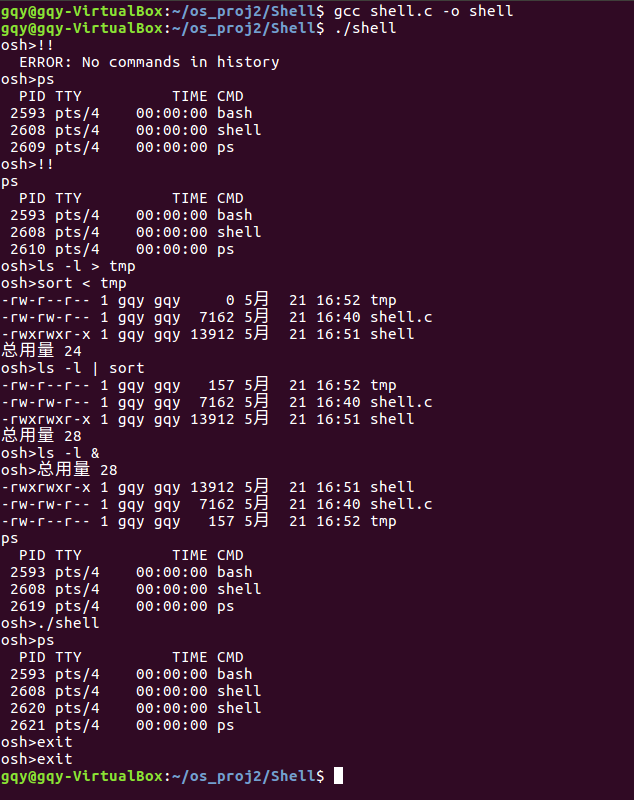
\includegraphics{shell}
		\caption{shell测试} \label{shell测试}%标题 自动编号 label标签
\end{figure}


测试指令如下
\begin{lstlisting}[language={[ANSI]C}]
gcc shell.c -o shell
./shell
!!
ps
!!
ls -l > tmp
sort < tmp
ls -l | sort
ls -l &
ps
./shell
ps
exit
exit
\end{lstlisting}
首先编译shell.c文件并执行,输入!!指令由于历史指令为空报错,之后正常执行ps指令,再输入!!指令就输出了历史指令ps并执行。然后ls -l > tmp和sort < tmp测试输入输出重定位,ls -l | sort测试pipe通信,ls -l \&测试并行。再次执行shell,然后输入ps可以看到当前系统任务列表有两层shell在执行,输入两次exit可以正常退出程序。
\end{itemize}

\section{Linux Kernel Module for Task Information}
\subsection{实验内容与目标}
\begin{itemize}
\item[$\bullet$]设计/proc文件系统内核模块
\item[$\bullet$]支持通过进程pid查看任务信息
\end{itemize}
\subsection{实验过程及步骤}
\begin{itemize}
\item[$\bullet$]读取用户输入的pid\\
首先模仿project1中的文件系统内核模块创建新的内核模块pid,根据书本指导,在file\_operations中增加.write = proc\_write语句,根据书本Figure 3.37创建proc\_write()函数。用kmalloc给k\_mem分配空间,用来存储user buffer的信息,在copy\_from\_user函数后增加k\_mem[count] = 0语句人为添加字符串结尾字符,否则会出现pid不合法的情况。使用kstrtol函数将k\_mem的信息传入pid,然后使用kfree释放空间。
\item[$\bullet$]根据pid列出任务信息\\
在proc\_read()函数中创建task\_struct类型的PCB,用pid\_task(find\_vpid(pid), PIDTYPE\_PID)来获取相应pid的PCB信息,并按格式输出任务信息然后copy\_to\_user。
\item[$\bullet$]应对不合法pid指令\\
如果pid\_task函数返回NULL,说明pid不合法,输出相应报错后退出。
\end{itemize}

\subsection{实验代码}
\begin{center}
{\ttfamily pid.c}
\end{center}
\begin{lstlisting}[language={[ANSI]C}]
# include <linux/init.h>
# include <linux/slab.h>
# include <linux/sched.h>
# include <linux/module.h>
# include <linux/kernel.h>
# include <linux/proc_fs.h>
# include <linux/vmalloc.h>
# include <linux/uaccess.h>
# include <asm/uaccess.h>

# define BUFFER_SIZE 128
# define PROC_NAME "pid"

static long pid;

static ssize_t proc_read(struct file *file, char *buf, size_t count, loff_t *pos);
static ssize_t proc_write(struct file *file, const char __user *usr_buf, size_t count, loff_t *pos);

static struct file_operations proc_ops = {
	.owner = THIS_MODULE,
	.read = proc_read,
	.write = proc_write,
};

static int proc_init(void) {

	proc_create(PROC_NAME, 0666, NULL, &proc_ops);
	printk(KERN_INFO "/proc/" PROC_NAME " is loaded!\n");
	return 0;
}

static void proc_exit(void) {

	remove_proc_entry(PROC_NAME, NULL);
	printk(KERN_INFO "/proc/" PROC_NAME " is removed!\n");
}

static ssize_t proc_read(struct file *file, char __user *usr_buf, size_t count, loff_t *pos) {
	int rv = 0;
	char buffer[BUFFER_SIZE];
	static int completed = 0;
	struct task_struct *PCB = NULL;

	if (completed) {
		completed = 0;
		return 0;
	}

	PCB = pid_task(find_vpid(pid), PIDTYPE_PID);
	if (PCB == NULL) {
		printk(KERN_INFO "Invalid PID!\n");
		return 0;
	}

	completed = 1;

	rv = sprintf(buffer, "command = [%s] pid = [%ld] state = [%ld]\n", PCB -> comm, pid, PCB -> state);
	
	copy_to_user(usr_buf, buffer, rv);

	return rv;
}

static ssize_t proc_write(struct file *file, const char __user *usr_buf, size_t count, loff_t *pos) 
{
	char *k_mem;

	// allocate kernel memory
	k_mem = kmalloc(count, GFP_KERNEL);

	// copies user space usr_buf to kernel buffer
	copy_from_user(k_mem, usr_buf, count);
	k_mem[count] = 0;

	kstrtol(k_mem, 10, &pid);

	// free the memory
	kfree(k_mem);

	return count;
}

module_init(proc_init);
module_exit(proc_exit);

MODULE_LICENSE("GPL");
MODULE_DESCRIPTION("Pid Module");
MODULE_AUTHOR("GQY");
\end{lstlisting}

\subsection{实验测试}
\begin{itemize}
\item[$\bullet$]pid测试 (图 \ref{pid测试})\\
\begin{figure}[htbp]%figure浮动体环境 [htbp]指定位置
		\centering%居中排版
		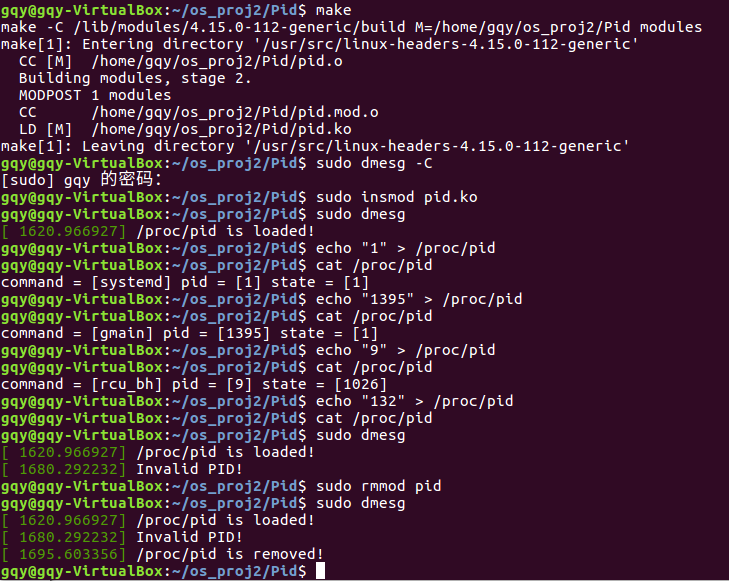
\includegraphics{pid}
		\caption{pid测试} \label{pid测试}%标题 自动编号 label标签
\end{figure}
测试指令如下
\begin{lstlisting}[language={[ANSI]C}]
make
sudo dmesg -C
sudo insmod pid.ko
sudo dmesg
echo "1" > /proc/pid
cat /proc/pid
echo "1395" > /proc/pid
cat /proc/pid
echo "9" > /proc/pid
cat /proc/pid
echo "132" > /proc/pid
cat /proc/pid
sudo dmesg
sudo rmmod pid
sudo dmesg
\end{lstlisting}
首先用Makefile文件编译内核模块,然后清空内核日志缓冲区并加载pid模块,输入dmesg可以看到内核模块成功加载。然后先后输入pid为1,1395,9查询,都可以通过cat /proc/pid正常看到任务信息,最后输入pid为132查询发现无法通过cat /proc/pid查询到任务信息,输入dmesg查看发现是因为pid不合法报错。最后卸载pid模块,输入dmesg可以看到内核模块成功卸载。
\end{itemize}

\section{Conclusion}

\subsection{问题与解决方案}
本次project2的UNIX shell部分稍有一点难度。首先分析指令部分需要对字符串操作比较熟悉;在设计支持重定位和pipe通信的时候遇到了许多新的函数,最开始并没有什么头绪,但是在仔细研读书本示例并经过多次尝试后最终成功完成。

project2的另一个部分pid内核模块的设计是project1延伸,书上的指导也比较细致,就是在设计proc\_write()函数的时候,如果仅仅根据书本上的操作会发现最后pid读取都非法,后来发现需要人为添加字符串结尾字符能避免该问题。

\subsection{实验心得}
本次project2是对所学知识一次很好的运用,比如设计UNIX shell需要有一个全局观念,要综合运用变量设计,空间分配,进程管理等方式,同时在实践的过程中也让我对pipe通信有了更深入的了解。虽然过程中也遇到了一些问题,但在耐心检查反复尝试的过程中都顺利解决了,总的来说本次project很好地锻炼了动手能力并加深了对理论知识的理解,让我受益匪浅。




%----------------------------------------------------------------------------------------


\end{document}